\section{Day 3}
\begin{tabular}{|c|c|}
\hline
Date: & 09.10.2013 \\
\hline
\end{tabular}
\subsection{First day at the office}
We were drown from our house to the ministry of health by Randy today. 08:30AM. Early day. Randy had some meetings and we've got the oppertunity to chack our emails and catch up on some reading. I found some new articles today that talked a little about how there is a gap between some countries in the IT world. Talked a little with Simen about ttrying to share our perspectives to get the best from both worlds.
\subsection{DHIS2 Intro}
After a while Randy was finished with his meetings. Andrew, the system wizard, came and said hello. He is joining us tomorrow for some DHIS2 training.
We where introduced to alot this session. Mostly about how they were using DHIS2 today. DHIS2 is not the only program they use. The functionality that are needed, but not supported by DHIS2, are hacked into their day-to-day work with some scripts made up by different people. I think their data is pushed to the server monthly. \\
Here is some changes that Randy suggested.
\begin{itemize}
\item Wanted to make some good validation rules, but lacked people with experience in the field to make them proparly.
\item After the usercount got high, the favorites got very messy and unorganized.
\item Would like to share tables, diagrammes and maps with individuals and make only a selected few public.
\item Some labels on the map, didnt quite get that one.
\item They would like to choose what type of faccilities that would be viewed in GIS. This would be a great improvement.
\item They had some language barriers. Would like som improbements there. Didnt get the details.
\item Problem with reports being loaded from NGINX cache, they were not updated after changes if it already was in NGINX cache.
\end{itemize} 
I was wondering how he trusted the data. It turned out that sometimes the data wasnt accurate. This was tested by some people motivated by a Performance Based Finance system. The health facilities down here get some funding based on their registration count. Some cases are worth more than others. Like, dont actually know the numbers, but lets say 1000RWF for registrating a pregnant woman. So to prevent health facilities from cheating the authoreties take some samples in order to check if the inputed data is correct. Randy would like some more competance on iReport. Should check that out later. FOSAID is the identification number used through all the databases. This identifies the facility. This number is also used by external systems. I think I should get a better understanding of Pivot tables. They are quite popular here. Camel is used to make an access level from the MOH to extarnal systems.\\
He also gave us an overview of how everything should be linked together in the future.\\
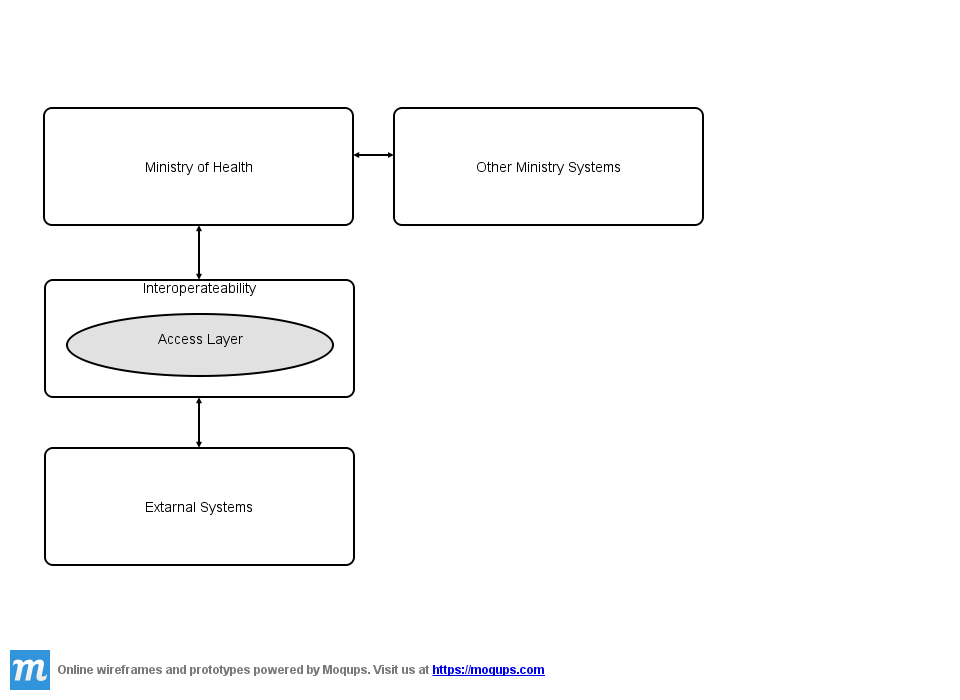
\includegraphics[width=15cm]{appendix/images/future_design_rwanda}\\
I then wondered how they could trust the open source code to do its job. Is there some testing that ensures that DHIS2 is working as it should? To me this seems like life or death for some people. When funding is based on registration of data. Is this the only option that MSH have? What other options did they consider before DHIS2? And what was the primary factor for choosing DHIS2. Open source? Proprietary softerware alternatives? I know I would be very sceptical to a software that did not guarantee customer support. 
\subsection{Lunch}
During luch we got some food from a burger diner. Good food, bad smell around the toilet. Randy just had a baby that is 4 months old with his second wife from Rwanda. She had family in Trondheim and visited them not to long ago. 
\subsection{Install Rwanda DHIS2}
When we got back we installed all the necesarry software. We got our own copy of the database so that we could work localy on our machines.
\begin{enumerate}
\item JDK
\item Postgres
\item Ireport
\item Tomcat
\item odbc
\item restore database
\item edit hibernate.properties
\end{enumerate}
I think I should get more comfortable with enviroment variables in Windows. 
I should get back to my todo list for sure.
\subsection{Dinner}
After work we ate at a Italian resturant. A little bit pricy. Should probably find some cheaper alternatives.
We are getting picked up at 07:30AM tomorrow, so I should probably get some sleep now. Good NIGHT!

